\subsection{Medida de Informação}
\begin{frame}%[allowframebreaks]
  \frametitle{Medida de Informação}
  Veremos as correspondências entre a medida de informação de Shannon (e suas manipulações)
  com a teoria de conjuntos. A utilização dos diagramas de informação podem ser utilizadas para 
  simplificar várias demonstrações em teoria da informação.
\end{frame}

\begin{frame}%[allowframebreaks]
  \frametitle{Medida de Informação}
  \begin{itemize}
  \item Temos um conjunto de variáveis aleatórias: $X_1, X_2, \ldots, X_n$.
  \item Para cada variável aleatória associamos um conjunto $\tilde{X}_1, \tilde{X}_2, \ldots, \tilde{X}_n$.
  \end{itemize}

  \begin{definition}[campo (field)]
  Um campo $\mathcal{F}_n$ gerado pelos conjuntos $\tilde{X}_1, \tilde{X}_2, \ldots, \tilde{X}_n$ é
  a coleção de conjuntos que podem ser obtidos através de qualquer sequência de operações
  usuais de conjuntos (união, interseção, complemento, e diferença) sobre os conjuntos 
  $\tilde{X}_1, \tilde{X}_2, \ldots, \tilde{X}_n$.
  \end{definition}

  \begin{definition}[átomo]
  Os átomos de $\mathcal{F}_n$ são os conjuntos da forma $\cap_{i=1}^n Y_i$, onde 
  $Y_i$ é $\tilde{X}_i$ ou $\tilde{X}_i^c$, o complemento de $\tilde{X}_i$.
  \end{definition}
\end{frame}

\begin{frame}%[allowframebreaks]
  \frametitle{Átomos}
  \begin{exampleblock}{átomos - $n=2$}
  Para $n=2$, teremos os conjuntos $\tilde{X}_1, \tilde{X}_2$ e seus complementos,
  respectivamente, $\tilde{X}_1^c, \tilde{X}_2^c$. Existirão $4$ átomos:

  \begin{minipage}[t]{0.35\linewidth}
  \begin{enumerate}
  \item $\tilde{X}_1 \cap \tilde{X}_2$,
  \item $\tilde{X}_1 \cap \tilde{X}_2^c$,
  \item $\tilde{X}_1^c \cap \tilde{X}_2$, e
  \item $\tilde{X}_1^c \cap \tilde{X}_2^c$
  \end{enumerate}
  \end{minipage} \hfill 
  \begin{minipage}[t]{0.55\linewidth}
    \begin{figure}[!ht]
    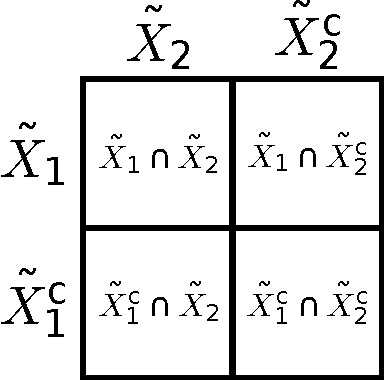
\includegraphics[width=0.5\linewidth]{images/atoms-n2.pdf}
    \end{figure}
  \end{minipage}

  \end{exampleblock}
\end{frame}

\begin{frame}%[allowframebreaks]
  \frametitle{Átomos}
  \begin{exampleblock}{átomos - $n=3$}
  Para $n=3$, teremos os conjuntos $\tilde{X}_1, \tilde{X}_2, \tilde{X}_3$ e seus complementos,  
  respectivamente, $\tilde{X}_1^c, \tilde{X}_2^c, \tilde{X}_3^c$. Existirão $8$ átomos:

  \begin{minipage}[t]{0.35\linewidth}
  \begin{enumerate}
  \item $\tilde{X}_1 \cap \tilde{X}_2 \cap \tilde{X}_3$,
  \item $\tilde{X}_1 \cap \tilde{X}_2 \cap \tilde{X}_3^c$,
  \item $\tilde{X}_1 \cap \tilde{X}_2^c \cap \tilde{X}_3$,
  \item $\tilde{X}_1 \cap \tilde{X}_2^c \cap \tilde{X}_3^c$,
  \item $\tilde{X}_1^c \cap \tilde{X}_2 \cap \tilde{X}_3$, 
  \item $\tilde{X}_1^c \cap \tilde{X}_2 \cap \tilde{X}_3^c$,
  \item $\tilde{X}_1^c \cap \tilde{X}_2^c \cap \tilde{X}_3$, e 
  \item $\tilde{X}_1^c \cap \tilde{X}_2^c \cap \tilde{X}_3^c$
  \end{enumerate}
  \end{minipage} \hfill
  \begin{minipage}[t]{0.6\linewidth}
    \begin{figure}[!ht]
    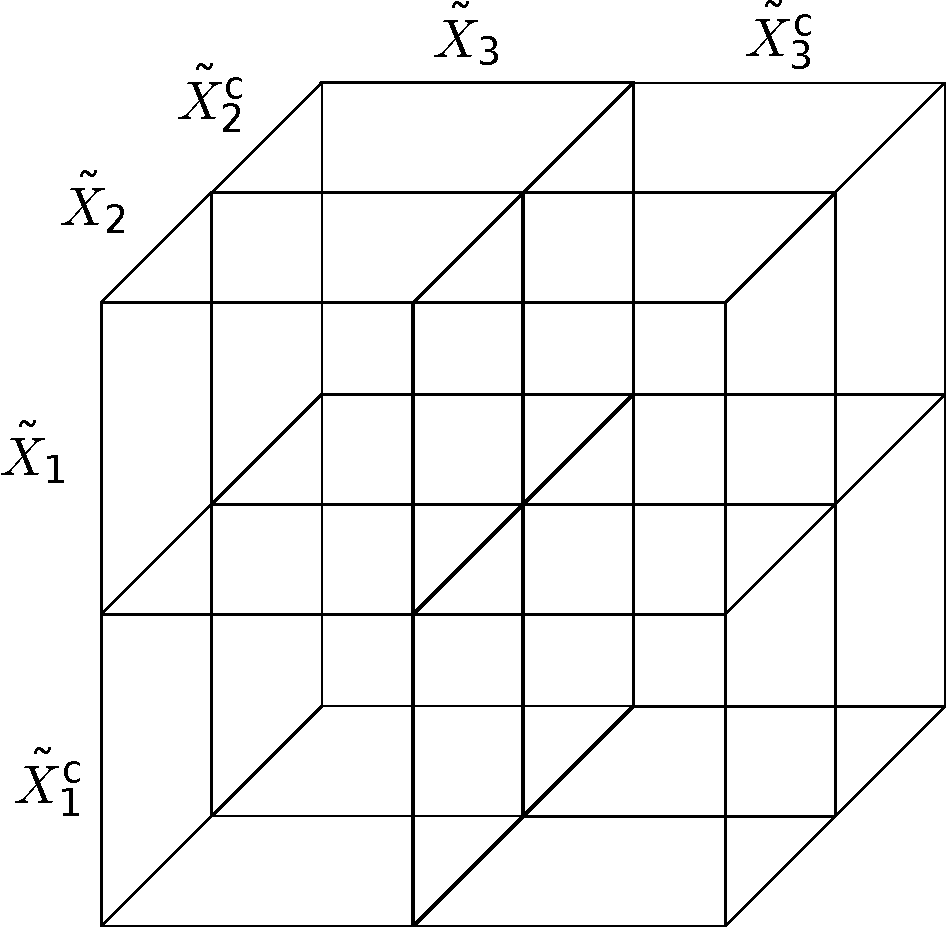
\includegraphics[width=0.6\linewidth]{images/atoms-n3.pdf}
    \end{figure}
  \end{minipage}

  \end{exampleblock}
\end{frame}

\begin{frame}%[allowframebreaks]
  \frametitle{Campo e Átomos}
  \begin{itemize}
  \item existem $2^n$ átomos;
  \item existem $2^{2^n}$ conjuntos no campo $\mathcal{F}_n$;
  \item todos os átomos em $\mathcal{F}_n$ são disjuntos;
  \item todo conjunto em $\mathcal{F}_n$ pode ser expresso de forma única como uma união de um subconjunto dos átomos em $\mathcal{F}_n$.
  \end{itemize}
\end{frame}

\begin{frame}%[allowframebreaks]
  \frametitle{Medida com sinal}
  Em análise matemática, uma medida em um conjunto $S$ é uma forma sistemática de atribuir
  números a todo subconjunto de $S$, sendo intuitivamente interpretada como o seu tamanho.

  Medida com sinal é uma generalização do conceito de medida permitindo que esta assuma valores
  negativos.

  \begin{definition}[medida com sinal]
  Uma função real $\mu$ definida em $\mathcal{F}_n$ é chamada medida com sinal se
  for aditiva no conjunto, i.e., para $A$ e $B$ disjuntos em $\mathcal{F}_n$,
  \begin{equation}
  \mu(A \cup B) = \mu(A) + \mu(B) .
  \end{equation} 
  \end{definition}  
  Para uma medida com sinal $\mu$ teremos $\mu(\emptyset)=0$, já que
  $\mu(A) = \mu(A \cup \emptyset) = \mu(A) + \mu(\emptyset)$.
\end{frame}

\begin{frame}%[allowframebreaks]
  \frametitle{Medida com sinal}
  Uma medida com sinal $\mu$ em $\mathcal{F}_n$ é completamente especificada
  por seus valores nos átomos de $\mathcal{F}_n$. Os valores de $\mu$ em outros
  conjuntos de $\mathcal{F}_n$ podem ser obtidos pela aditividade de conjuntos, 
  já que qualquer $\tilde{X} \in \mathcal{F}_n$ pode ser representado como
  $\tilde{X} = \cup_{i=1} Y_i$, onde $Y_i$ são átomos escolhidos apropriadamente.
\end{frame}


\begin{frame}%[allowframebreaks]
  \frametitle{Medida com sinal}
  \begin{exampleblock}{$n=2$}
  Uma medida com sinal $\mu$ em $\mathcal{F}_2$ é completamente especificada pelos
  valores 
  $\mu( \tilde{X}_1 \cap \tilde{X}_2 )$,
  $\mu( \tilde{X}_1 \cap \tilde{X}_2^c )$,
  $\mu( \tilde{X}_1^c \cap \tilde{X}_2 )$, e
  $\mu( \tilde{X}_1^c \cap \tilde{X}_2^c )$.

  O valor de $\mu$ em $\tilde{X}_1$ pode ser obtido da seguinte forma
  \begin{eqnarray}
  \mu( \tilde{X}_1 ) &=& \mu( (\tilde{X}_1 \cap \tilde{X}_2) \cup ( \tilde{X}_1 \cap \tilde{X}_2^c) ) \nonumber \\
		&=& \mu( \tilde{X}_1 \cap \tilde{X}_2 ) + \mu( \tilde{X}_1 \cap \tilde{X}_2^c ) .
  \end{eqnarray}

  O valor de $\mu$ em $\tilde{X}_1 \setminus \tilde{X}_2$ é dado por
  \begin{equation}
  \mu( \tilde{X}_1 \setminus \tilde{X}_2 ) = \mu( \tilde{X}_1 \cap \tilde{X}_2^c ) .
  \end{equation}

  O valor de $\mu$ em $\tilde{X}_1 \cup \tilde{X}_2$ pode ser obtido através de
  \begin{eqnarray}
  \mu( \tilde{X}_1 \cup \tilde{X}_2 ) &=& \mu( (\tilde{X}_1 \cap \tilde{X}_2) \cup (\tilde{X}_1 \cap \tilde{X}_2^c) \cup (\tilde{X}_1^c \cap \tilde{X}_2) ) \nonumber \\
	&=& \mu( \tilde{X}_1 \cap \tilde{X}_2 ) + \mu( \tilde{X}_1 \cap \tilde{X}_2^c ) + \mu(\tilde{X}_1^c \cap \tilde{X}_2) 
  \end{eqnarray}

  \end{exampleblock}
\end{frame}


\begin{frame}[allowframebreaks]
  \frametitle{Correspondência com a informação de Shannon}
  Os conjuntos $\tilde{X}_1$ e $\tilde{X}_2$ estão associados às variáveis
  aleatória $X_1$ e $X_2$. O campo $\mathcal{F}_2$ é gerado por $\tilde{X}_1$ e $\tilde{X}_2$,
  através dos átomos 
  $(\tilde{X}_1 \cap \tilde{X}_2)$,
  $(\tilde{X}_1 \cap \tilde{X}_2^c)$,
  $(\tilde{X}_1^c \cap \tilde{X}_2)$, e
  $(\tilde{X}_1^c \cap \tilde{X}_2^c)$.
  O diagrama de informação é apresentado na Figura \ref{fig:setX1X2}.

  \begin{figure}[h!]
  \centering
  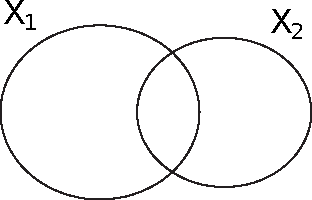
\includegraphics[width=0.4\textwidth]{images/setX1X2.pdf}
  \caption{Diagrama de informação para $X_1$ e $X_2$.}
  \label{fig:setX1X2}
  \end{figure}
 
  O conjunto universo será considerada como sendo $\Omega = \tilde{X}_1 \cup \tilde{X}_2$.
  Desta forma, o átomo $\tilde{X}_1^c \cap \tilde{X}_2^c$ se degenera ao conjunto vazio,
  \begin{equation}
  \tilde{X}_1^c \cap \tilde{X}_2^c = (\tilde{X}_1 \cup \tilde{X}_2)^c = \Omega^c = \emptyset .
  \end{equation}

  Para as v.a.s $X_1$ e $X_2$, as medidas de informação de Shannon são 
  \begin{equation}
  H(X_1), H(X_2), H(X_1|X_2), H(X_2|X_1), H(X_1,X_2), I(X_1;X_2) .
  \end{equation}

  Utilizando a notação $A \cap B^c \equiv A \setminus B$, definimos uma medida com sinal $\mu^\ast$
  \begin{eqnarray}
  \mu^\ast(\tilde{X}_1 \setminus \tilde{X}_2) &=& H(X_1|X_2) ,\\
  \mu^\ast(\tilde{X}_2 \setminus \tilde{X}_1) &=& H(X_2|X_1) ,\\
  \mu^\ast(\tilde{X}_1 \cap \tilde{X}_2) &=& I(X_1;X_2) .
  \end{eqnarray}
  Estes são os valores de $\mu^\ast$ nos átomos não vazios de $\mathcal{F}_2$.
  Os valores de $\mu^\ast$ nos demais conjuntos de $\mathcal{F}_2$ podem ser obtidos por
  adição de conjuntos. Em particular, temos as relações
  \begin{eqnarray}
  \mu^\ast(\tilde{X}_1 \cup \tilde{X}_2) &=& H(X_1, X_2) , \label{eqX1X2HX1X2} \\
  \mu^\ast(\tilde{X}_1) &=& H(X_1) , \label{eqmuX1HX1}\\
  \mu^\ast(\tilde{X}_2) &=& H(X_2) .
  \end{eqnarray}

  Por exemplo, a Equação \ref{eqX1X2HX1X2} pode ser verificada
  \begin{eqnarray}
  \mu^\ast(\tilde{X}_1 \cup \tilde{X}_2) &=& \mu^\ast( (\tilde{X}_1 \setminus \tilde{X}_2) \cup (\tilde{X}_2 \setminus \tilde{X}_1) \cup (\tilde{X}_1 \cap \tilde{X}_2) ) \nonumber \\
	&=& \mu^\ast( \tilde{X}_1 \setminus \tilde{X}_2 ) + \mu^\ast( \tilde{X}_2 \setminus \tilde{X}_1 ) + \mu^\ast( \tilde{X}_1 \cap \tilde{X}_2 ) \nonumber \\
	&=& H(X_1|X_2) + H(X_2|X_1) + I(X_1;X_2) \nonumber \\
	&=& H(X_1, X_2) .
  \end{eqnarray}

  A Equação \ref{eqmuX1HX1} também pode ser facilmente verificada
  \begin{eqnarray}
  \mu^\ast(\tilde{X}_1) &=& \mu^\ast( (\tilde{X}_1 \cap \tilde{X}_2) \cup (\tilde{X}_1 \cap \tilde{X}_2^c) ) \nonumber \\
	&=& \mu^\ast(\tilde{X}_1 \cap \tilde{X}_2) + \mu^\ast(\tilde{X}_1 \cap \tilde{X}_2^c) \nonumber \\
	&=& I(X_1;X_2) + H(X_1|X_2) = H(X_1) .
  \end{eqnarray}

  É possível então verificar a seguinte correspondência com as medidas de informação de Shannon
  \begin{eqnarray}
  H / I &\leftrightarrow& \mu^\ast \\
  , &\leftrightarrow& \cup \\
  ; &\leftrightarrow& \cap \\
  | &\leftrightarrow& \setminus 
  \end{eqnarray}

  \begin{itemize}
  \item obs.: com a notação de medida, não existe distinção entre $H$ e $I$, podemos escrever
	$H(X;Y) = I(X;Y)$, utilizando a notação do ponto-e-vírgula.
  \end{itemize}
\end{frame}


